\documentclass[8pt,a4paper,compress,handout]{beamer}

\usepackage{/home/siyer/lib/slides}

\title{Using Data Types}
\date{}

\begin{document}
\begin{frame}
\vfill
\titlepage
\end{frame}

\begin{frame}
\frametitle{Outline}
\tableofcontents
\end{frame}

\section{Methods}
\begin{frame}[fragile]
A \emph{method} is a function associated with a specific object (and, by extension, with the type of that object)

\bigskip

A method corresponds to a data-type operation

\bigskip

We \emph{call} (or \emph{invoke}) a method using a variable name, followed by the dot operator (\lstinline{.}), followed by the method name, followed by its arguments separated by commas and enclosed in parentheses

\begin{lstlisting}[language={}]
x = 3 ** 100
bits = x.bit_length()
stdio.writeln(bits)
\end{lstlisting}
\end{frame}

\section{Integers, Floats, Booleans, and Strings}
\begin{frame}[fragile]
Methods in the built-in \lstinline{int} data type
\begin{lstlisting}[language={}]
>>> dir(int) 
['bit_length', 'conjugate', 'denominator', 'imag', 'numerator', 'real']
\end{lstlisting}

\bigskip

Methods in the built-in \lstinline{float} data type
\begin{lstlisting}[language={}]
>>> dir(float) 
['as_integer_ratio', 'conjugate', 'fromhex', 'hex', 'imag', 'is_integer', 
 'real']
\end{lstlisting}

\bigskip

Methods in the built-in \lstinline{bool} data type
\begin{lstlisting}[language={}]
>>> dir(bool) 
['bit_length', 'conjugate', 'denominator', 'imag', 'numerator', 'real']
\end{lstlisting}

\bigskip

Methods in the built-in \lstinline{str} data type
\begin{lstlisting}[language={}]
>>> dir(str)
['capitalize', 'center', 'count', 'decode', 'encode', 'endswith', 'expandtabs', 
 'find', 'format', 'index', 'isalnum', 'isalpha', 'isdigit', 'islower', 
 'isspace', 'istitle', 'isupper', 'join', 'ljust', 'lower', 'lstrip', 
 'partition', 'replace', 'rfind', 'rindex', 'rjust', 'rpartition', 
 'rsplit', 'rstrip', 'split', 'splitlines', 'startswith', 'strip', 
 'swapcase', 'title', 'translate', 'upper', 'zfill']
\end{lstlisting}
\end{frame}

\begin{frame}[fragile]
\begin{framed}
\tiny potentialgene.py: Accepts a DNA sequence as a command-line argument, and writes \lstinline{True} to standard output if the sequence corresponds to a potential gene, and \lstinline{False} otherwise.
\end{framed}

\begin{lstlisting}[language=Python]
import stdio
import sys

def isPotentialGene(dna):
    if (len(dna) % 3) != 0: return False
    if not dna.startswith('ATG'): return False
    for i in range(len(dna) - 3):
        if i % 3 == 0:
            if dna[i:i + 3] == 'TAA': return False
            if dna[i:i + 3] == 'TAG': return False
            if dna[i:i + 3] == 'TGA': return False
    if dna.endswith('TAA'): return True
    if dna.endswith('TAG'): return True
    if dna.endswith('TGA'): return True
    return False

def main():
    dna = sys.argv[1]
    stdio.writeln(isPotentialGene(dna))

if __name__ == '__main__':
    main()
\end{lstlisting}

\begin{lstlisting}[language={}]
$ python potentialgene.py ATGCGCCTGCGTCTGTACTAG
True
$ python potentialgene.py ATGCGCTGCGTCTGTACTAG
False
\end{lstlisting}
\end{frame}

\section{Collections}
\begin{frame}[fragile]
Methods in the built-in \lstinline{list} data type
\begin{lstlisting}[language={}]
>>> dir(list)
['append', 'count', 'extend', 'index', 'insert', 'pop', 'remove', 'reverse', 
 'sort']
\end{lstlisting}

\bigskip

Methods in the built-in \lstinline{tuple} data type
\begin{lstlisting}[language={}]
>>> dir(tuple)
['count', 'index']
\end{lstlisting}

\bigskip

Methods in the built-in \lstinline{set} data type
\begin{lstlisting}[language={}]
>>> dir(set)
['add', 'clear', 'copy', 'difference', 'difference_update', 'discard', 
 'intersection', 'intersection_update', 'isdisjoint', 'issubset', 
 'issuperset', 'pop', 'remove', 'symmetric_difference',  
 'symmetric_difference_update', 'union', 'update']
\end{lstlisting}

\bigskip

Methods in the built-in \lstinline{dict} data type
\begin{lstlisting}[language={}]
>>> dir(dict)
['clear', 'copy', 'fromkeys', 'get', 'has_key', 'items', 'iteritems', 
 'iterkeys', 'itervalues', 'keys', 'pop', 'popitem', 'setdefault', 'update', 
 'values', 'viewitems', 'viewkeys', 'viewvalues']
\end{lstlisting}
\end{frame}

\section{User-Defined Data Types}
\begin{frame}[fragile]
A data type \lstinline{Charge} for charged particles
\begin{center}
\begin{tabular}{cc}
method & description \\ \hline
\lstinline$Charge(x0, y0, q0)$ & a new charge $c$ centered at $(x_0, y_0)$ with charge value $q_0$ \\
\lstinline$c.potentialAt(x, y)$ & electric potential of charge $c$ at point $(x, y)$ \\
\lstinline$str(c)$ & string representation of charge $c$
\end{tabular} 
\end{center}

\bigskip

To create an object of a user-defined data type, we call its \emph{constructor}, using the name of the data type, followed by the constructor's arguments

\bigskip

We use a variable name to identify the object to be associated with the method we intend to call

\bigskip

In any data-type implementation, it is worthwhile to include an operation that converts an object's value to a string

\bigskip

We will use the following form of the \lstinline{import} statement to import a data type \lstinline{XYZ} defined in a file \lstinline{xyz.py}
\begin{lstlisting}[language={}]
from xyz import XYZ
\end{lstlisting}
\end{frame}

\begin{frame}[fragile]
\begin{framed}
\tiny chargeclient.py: Accepts floats $x$ and $y$ as command-line arguments, creates two \lstinline{Charge} objects with fixed position and electrical charge, and writes to standard output the potential at $(x, y)$ due to the two charges.
\end{framed}

\begin{lstlisting}[language=Python]
import stdio
import sys
from charge import Charge

def main():
    x = float(sys.argv[1])
    y = float(sys.argv[2])
    c1 = Charge(.51, .63, 21.3)
    c2 = Charge(.13, .94, 81.9)
    v1 = c1.potentialAt(x, y)
    v2 = c2.potentialAt(x, y)
    stdio.writef('potential at (%.2f, %.2f) due to\n', x, y)
    stdio.writeln('  ' + str(c1) + ' and')
    stdio.writeln('  ' + str(c2))
    stdio.writef('is %.2e\n', v1 + v2)

if __name__ == '__main__':
    main()
\end{lstlisting}

\begin{lstlisting}[language={}]
$ python chargeclient.py .2 .5
potential at (0.20, 0.50) due to
  21.3 at (0.51, 0.63) and
  81.9 at (0.13, 0.94)
is 2.22e+12
$ python chargeclient.py .51 .94
potential at (0.51, 0.94) due to
  21.3 at (0.51, 0.63) and
  81.9 at (0.13, 0.94)
is 2.56e+12
\end{lstlisting}
\end{frame}

\begin{frame}[fragile]
A data type \lstinline{Color} for representing color values
\begin{center}
\begin{tabular}{cc}
method & description \\ \hline
\lstinline$Color(r, g, b)$ & \makecell{a new color $c$ with red, green, and blue components \\ $r$, $g$, and $b$, all integers between 0 and 255} \\
\lstinline$c.getRed()$ & the red component of $c$ \\
\lstinline$c.getGreen()$ & the green component of $c$ \\
\lstinline$c.getBlue()$ & the blue component of $c$ \\
\lstinline$str(c)$ & string representation of $c$
\end{tabular} 
\end{center}
\end{frame}

\begin{frame}[fragile]
\begin{framed}
\tiny alberssquares.py: Accepts integers $r1$, $g1$, $b1$, $r2$, $g2$, and $b2$ as command-line arguments, and draws to standard draw Albers squares using colors $(r1, g1, b1)$ and $(r2, g2, b2)$.
\end{framed}

\begin{lstlisting}[language=Python]
import stddraw
import sys
from color import Color

def main():
    r1 = int(sys.argv[1])
    g1 = int(sys.argv[2])
    b1 = int(sys.argv[3])
    c1 = Color(r1, g1, b1)
    r2 = int(sys.argv[4])
    g2 = int(sys.argv[5])
    b2 = int(sys.argv[6])
    c2 = Color(r2, g2, b2)
    stddraw.setCanvasSize(512, 256)
    stddraw.setYscale(.25, .75)
    stddraw.setPenColor(c1)
    stddraw.filledSquare(.25, .5, .2)
    stddraw.setPenColor(c2)
    stddraw.filledSquare(.25, .5, .1)
    stddraw.setPenColor(c2)
    stddraw.filledSquare(.75, .5, .2)
    stddraw.setPenColor(c1)
    stddraw.filledSquare(.75, .5, .1)
    stddraw.show()

if __name__ == '__main__':
    main()
\end{lstlisting}
\end{frame}

\begin{frame}[fragile]
\begin{minipage}{180pt}
\begin{lstlisting}[language={}]
$ python alberssquares.py 9 90 166 100 100 100
\end{lstlisting}
\end{minipage}%
\hfill
\begin{minipage}{120pt}
\begin{center}
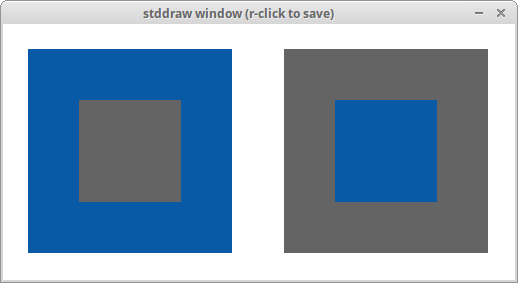
\includegraphics[scale=0.17]{figures/albers1.png}

\smallskip

\tiny Albers squares using colors $(9, 90, 166)$ and $(100, 100, 100)$
\end{center}
\end{minipage}

\bigskip

\begin{minipage}{180pt}
\begin{lstlisting}[language={}]
$ python alberssquares.py 0 174 239 147 149 252
\end{lstlisting}
\end{minipage}%
\hfill
\begin{minipage}{120pt}
\begin{center}
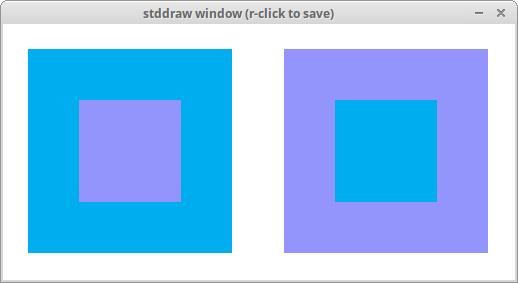
\includegraphics[scale=0.17]{figures/albers2.png}

\smallskip

\tiny Albers squares using colors $(0, 174, 239)$ and $(147, 149, 252)$
\end{center}
\end{minipage}
\end{frame}

\begin{frame}[fragile]
\begin{framed}
\tiny luminance.py: Accepts six RGB values defining two colors as command-line arguments, and writes \lstinline{True} to standard output if the two colors are compatible, and \lstinline{False} otherwise.
\end{framed}

\begin{lstlisting}[language=Python]
import stdio
import sys
from color import Color

def luminance(c):
    red   = c.getRed()
    green = c.getGreen()
    blue  = c.getBlue()
    return (.299 * red) + (.587 * green) + (.114 * blue)

def toGray(c):
    y = int(round(luminance(c)))
    return Color(y, y, y)

def areCompatible(c1, c2):
    return abs(luminance(c1) - luminance(c2)) >= 128.0

def main():
    r1 = int(sys.argv[1])
    g1 = int(sys.argv[2])
    b1 = int(sys.argv[3])
    r2 = int(sys.argv[4])
    g2 = int(sys.argv[5])
    b2 = int(sys.argv[6])
    c1 = Color(r1, g1, b1)
    c2 = Color(r2, g2, b2)
    stdio.writeln(areCompatible(c1, c2))

if __name__ == '__main__':
    main()
\end{lstlisting}
\end{frame}

\begin{frame}[fragile]
\begin{lstlisting}[language={}]
$ python luminance.py 232 232 232 0 0 0
True
$ python luminance.py 9 90 166 232 232 232
True
$ python luminance.py 9 90 166 0 0 0
False
\end{lstlisting}
\end{frame}

\begin{frame}[fragile]
A data type \lstinline{Picture} for representing digital images
\begin{center}
\begin{tabular}{cc}
method & description \\ \hline
\lstinline$Picture(w, h)$ & a new $w$-by-$h$ picture $pic$ \\
\lstinline$Picture(filename)$ & a new picture $pic$ initialized from $filename$ \\
\lstinline$pic.save(filename)$ & save $pic$ to $filename$ \\
\lstinline$pic.width()$ & the width of $pic$ \\
\lstinline$pic.height()$ & the height of $pic$ \\
\lstinline$pic.get(col, row)$ & the color of pixel $(col, row)$ in $pic$ \\
\lstinline$pic.set(col, row, c)$ & set the color of pixel $(col, row)$ in $pic$ to $c$
\end{tabular} 
\end{center}
\end{frame}

\begin{frame}[fragile]
\begin{framed}
\tiny grayscale.py: Accepts the name of a JPG or PNG file as a command-line argument, reads an image from the file, and draws a gray scale version of that image to standard draw.
\end{framed}

\begin{lstlisting}[language=Python]
import luminance
import stddraw
import sys
from picture import Picture

def main():
    pic = Picture(sys.argv[1])
    for col in range(pic.width()):
        for row in range(pic.height()):
            pixel = pic.get(col, row)
            gray = luminance.toGray(pixel)
            pic.set(col, row, gray)
    stddraw.setCanvasSize(pic.width(), pic.height())
    stddraw.picture(pic)
    stddraw.show()

if __name__ == '__main__':
    main()
\end{lstlisting}

\begin{minipage}{200pt}
\begin{lstlisting}[language={}]
$ python grayscale.py mandrill.jpg
\end{lstlisting}
\end{minipage}%
\hfill
\begin{minipage}{100pt}
\begin{center}
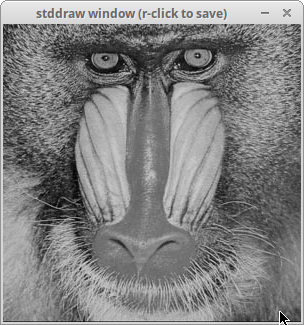
\includegraphics[scale=0.2]{figures/grayscale.png}

\smallskip

\tiny Mandrill image in gray scale
\end{center}
\end{minipage}
\end{frame}

\begin{frame}[fragile]
\begin{framed}
\tiny scale.py: Accepts the name $fileName$ of a JPG or PNG image file, an integer $w$, and an integer $h$ as command line arguments, reads an image from the file, and draws to standard draw the image scaled to width $w$ and height $h$.
\end{framed}

\begin{lstlisting}[language=Python]
import stddraw
import sys
from picture import Picture

def main():
    fileName = sys.argv[1]
    w = int(sys.argv[2])
    h = int(sys.argv[3])
    source = Picture(fileName)
    target = Picture(w, h)
    for tCol in range(w):
        for tRow in range(h):
            sCol = tCol * source.width() // w
            sRow = tRow * source.height() // h
            target.set(tCol, tRow, source.get(sCol, sRow))
    stddraw.setCanvasSize(w, h)
    stddraw.picture(target)
    stddraw.show()

if __name__ == '__main__':
    main()
\end{lstlisting}
\end{frame}

\begin{frame}[fragile]
\begin{minipage}{200pt}
\begin{lstlisting}[language={}]
$ python scale.py mandrill.jpg 200 200
\end{lstlisting}
\end{minipage}%
\hfill
\begin{minipage}{100pt}
\begin{center}
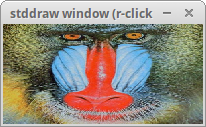
\includegraphics[width=2.5cm,height=2.5cm]{figures/scale2.png}

\smallskip

\tiny Mandrill image (200-by-200)
\end{center}
\end{minipage}%

\bigskip

\begin{minipage}{200pt}
\begin{lstlisting}[language={}]
$ python scale.py mandrill.jpg 200 100
\end{lstlisting}
\end{minipage}%
\hfill
\begin{minipage}{100pt}
\begin{center}
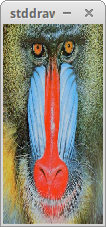
\includegraphics[width=2.5cm,height=1.25cm]{figures/scale3.png}

\smallskip

\tiny Mandrill image (200-by-100)
\end{center}
\end{minipage}%

\bigskip

\begin{minipage}{200pt}
\begin{lstlisting}[language={}]
$ python scale.py mandrill.jpg 100 200
\end{lstlisting}
\end{minipage}%
\hfill
\begin{minipage}{100pt}
\begin{center}
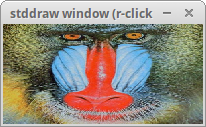
\includegraphics[width=1.25cm,height=2.5cm]{figures/scale1.png}

\smallskip

\tiny Mandrill image (100-by-200)
\end{center}
\end{minipage}%
\end{frame}

\begin{frame}[fragile]
\begin{framed}
\tiny fade.py: Accepts strings $sourceFile$ and $targetFile$ and integer $n$ as command-line arguments, and then, over the course of $n$ frames, gradually replaces the image from $sourceFile$ with the image from $targetFile$, and displays to standard draw each intermediate image. 
\end{framed}

\begin{lstlisting}[language=Python]
import stddraw
import sys
from color import Color
from picture import Picture

def blend(c1, c2, alpha):
    r = (1 - alpha) * c1.getRed()   + alpha * c2.getRed()
    g = (1 - alpha) * c1.getGreen() + alpha * c2.getGreen()
    b = (1 - alpha) * c1.getBlue()  + alpha * c2.getBlue()
    return Color(int(r), int(g), int(b))

def main():
    sourceFile = sys.argv[1]
    targetFile = sys.argv[2]
    n = int(sys.argv[3])
    source = Picture(sourceFile)
    target = Picture(targetFile)
    width = source.width()
    height = source.height()
    stddraw.setCanvasSize(width, height)
    pic = Picture(width, height)
\end{lstlisting}
\end{frame}

\begin{frame}[fragile]
\begin{lstlisting}[language=Python]
    for t in range(n + 1):
        for col in range(width):
            for row in range(height):
                c0 = source.get(col, row)
                cn = target.get(col, row)
                alpha = float(t) / float(n)
                c = blend(c0, cn, alpha)
                pic.set(col, row, c)
        stddraw.picture(pic)
        stddraw.show(1000.0)
    stddraw.show()

if __name__ == '__main__':
    main()
\end{lstlisting}

\begin{lstlisting}[language={}]
$ python fade.py mandrill.jpg darwin.jpg 5
\end{lstlisting}
\begin{minipage}{300pt}
\begin{center}
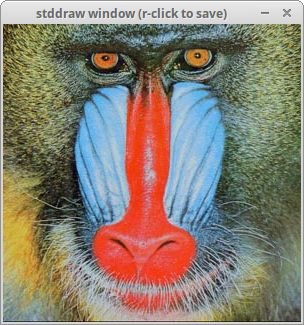
\includegraphics[scale=0.15]{figures/fade1.png}\hfill
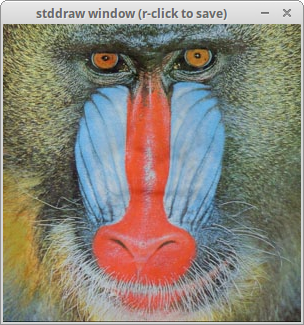
\includegraphics[scale=0.15]{figures/fade2.png}\hfill
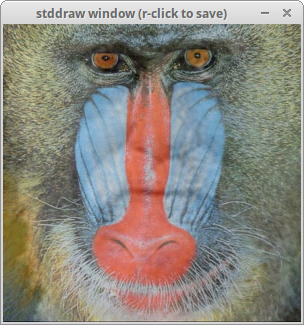
\includegraphics[scale=0.15]{figures/fade3.png}\hfill
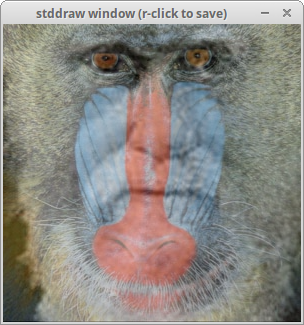
\includegraphics[scale=0.15]{figures/fade4.png}\hfill
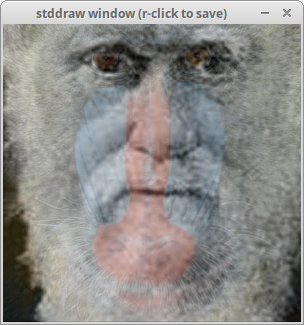
\includegraphics[scale=0.15]{figures/fade5.png}\hfill
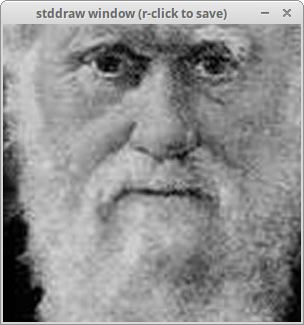
\includegraphics[scale=0.15]{figures/fade6.png}

\smallskip

\tiny Mandrill image faded into Darwin image over 5 frames
\end{center}
\end{minipage}%
\end{frame}

\begin{frame}[fragile]
\begin{framed}
\tiny potential.py: Reads values from standard input to create a list of charged particles, sets each pixel color in an image to a grayscale value proportional to the potential due to the particles at corresponding points, and draws the resulting image to standard draw.
\end{framed}

\begin{lstlisting}[language=Python]
import stdarray
import stddraw
import stdio
from charge import Charge
from color import Color
from picture import Picture

def main():
    MAX_GRAY_SCALE = 255
    WIDTH  = 512
    HEIGHT = 512
    n = stdio.readInt()
    charges = stdarray.create1D(n)
    for i in range(n):
        x0 = stdio.readFloat()
        y0 = stdio.readFloat()
        q0 = stdio.readFloat()
        charges[i] = Charge(x0, y0, q0)
    pic = Picture(WIDTH, HEIGHT)
    for col in range(pic.width()):
        for row in range(pic.height()):
            x = 1.0 * col / pic.width()
            y = 1.0 * row / pic.height()
            v = 0.0
            for i in range(n):
                v += charges[i].potentialAt(x, y)    
\end{lstlisting}
\end{frame}

\begin{frame}[fragile]
\begin{lstlisting}[language=Python]
            v = (MAX_GRAY_SCALE / 2.0)  + (v / 2.0e10)
            if v < 0:
                grayScale = 0
            elif v > MAX_GRAY_SCALE:
                grayScale = MAX_GRAY_SCALE
            else:
                grayScale = int(v)            
            color = Color(grayScale, grayScale, grayScale)
            pic.set(col, pic.height() - 1 - row, color)
    stddraw.setCanvasSize(pic.width(), pic.height())
    stddraw.picture(pic)
    stddraw.show()

if __name__ == '__main__':
    main()
\end{lstlisting}
\begin{minipage}{150pt}
\begin{lstlisting}[language={}]
$ more charges.txt
9
.51 .63 -100
.50 .50   40
.50 .72   10
.33 .33    5
.20 .20  -10
.70 .70   10
.82 .72   20
.85 .23   30
.90 .12  -50
$ python potential.py < charges.txt
\end{lstlisting}
\end{minipage}%
\hfill
\begin{minipage}{150pt}
\begin{center}
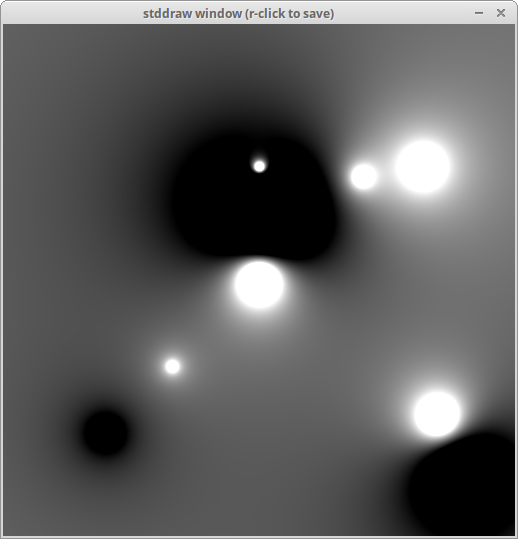
\includegraphics[scale=0.2]{figures/potential.png}

\smallskip

\tiny Electric potential visualized
\end{center}
\end{minipage}
\end{frame}

\begin{frame}[fragile]
A data type \lstinline{InStream} that supports reading numbers and text from files and websites as well as the standard input
\begin{center}
\begin{tabular}{cc}
method & description \\ \hline
\lstinline$InStream(filename)$ & \makecell{a new input stream $in$, initialized \\ from $filename$ (defaults to standard input)} \\
\lstinline$in.isEmpty()$ & is $in$ empty? \\
\lstinline$in.readInt()$ & read a token from $in$, and return it as an integer \\
\lstinline$in.readFloat()$ & read a token from $in$, and return it as a float \\
\lstinline$in.readBool()$ & read a token from $in$, and return it as a boolean \\
\lstinline$in.readString()$ & read a token from $in$, and return it as a string \\
$\dots$ & $\dots$
\end{tabular} 
\end{center}

\bigskip

A data type \lstinline{OutStream} that supports writing strings to a variety of output streams, including standard output and files
\begin{center}
\begin{tabular}{cc}
method & description \\ \hline
\lstinline$OutStream(filename)$ & \makecell{a new output stream $out$ that will write \\ to $filename$ (defaults to standard output)} \\
\lstinline$out.write(x)$ & write $x$ to $out$ \\
\lstinline$out.writeln(x)$ & write $x$ to $out$, followed by a newline \\
\lstinline$out.writef(fmt, arg1, ...)$ & \makecell{write the arguments $arg_1$, $\dots$ to $out$ as \\ specified by the format string $fmt$}
\end{tabular} 
\end{center}
\end{frame}

\begin{frame}[fragile]
\begin{framed}
\tiny cat.py: Copies files or web pages whose names are given by \lstinline{sys.argv[1:n - 2]} to the file whose name is given by \lstinline{sys.argv[n - 1]}.
\end{framed}

\begin{lstlisting}[language=Python]
import sys
from instream import InStream
from outstream import OutStream

def main():
    inFilenames = sys.argv[1:len(sys.argv) - 1]
    outFilename = sys.argv[len(sys.argv) - 1]
    outstream = OutStream(outFilename)
    for filename in inFilenames:
        instream = InStream(filename)
        s = instream.readAll()
        outstream.write(s)

if __name__ == '__main__':
    main()
\end{lstlisting}

\begin{lstlisting}[language={}]
$ more in1.txt
This is
$ more in2.txt
a tiny
test.
$ python cat.py in1.txt in2.txt out.txt
$ more out.txt
This is
a tiny
test.
\end{lstlisting}
\end{frame}

\begin{frame}[fragile]
\begin{framed}
\tiny stockquote.py: Accepts string $stockSymbol$ as a command-line argument, and writes to standard output the current stock price for $stockSymbol$, as reported by the website \href{http://finance.yahoo.com/}{http://finance.yahoo.com/}.
\end{framed}

\begin{lstlisting}[language=Python]
import stdio
import sys
from instream import InStream

def _readHTML(stockSymbol):
    WEBSITE = 'http://finance.yahoo.com/q?s='
    page = InStream(WEBSITE + stockSymbol)
    html = page.readAll()
    return html

def priceOf(stockSymbol):
    html  = _readHTML(stockSymbol)
    trade = html.find('yfs_l84', 0)
    beg   = html.find('>', trade)
    end   = html.find('</span>', beg)
    price = html[beg+1:end]
    price = price.replace(',', '')
    return float(price)

def main():
    stockSymbol = sys.argv[1]
    price = priceOf(stockSymbol)
    stdio.writef('%.2f\n', price)

if __name__ == '__main__':
    main()
\end{lstlisting}

\begin{lstlisting}[language={}]
$ python stockquote.py goog
733.76
\end{lstlisting}
\end{frame}

\begin{frame}[fragile]
\begin{framed}
\tiny split.py: Accepts string $fileName$ and integer $fieldCount$ as command-line arguments, splits the file whose name is \lstinline{fileName.csv}, by field, into $fieldCount$ files named \lstinline{fileName0.txt}, \lstinline{fileName1.txt}, etc.
\end{framed}

\begin{lstlisting}[language=Python]
import stdarray
import sys
from instream import InStream
from outstream import OutStream

def main():
    DELIM = ','
    fileName = sys.argv[1]
    fieldCount = int(sys.argv[2])
    inStream = InStream(fileName + '.csv')
    outStreams = stdarray.create1D(fieldCount)
    for i in range(fieldCount):
        outStreams[i] = OutStream(fileName + str(i) + '.txt')
    while inStream.hasNextLine():
        line = inStream.readLine()
        fields = line.split(DELIM)
        for i in range(fieldCount):
            outStreams[i].writeln(fields[i])

if __name__ == '__main__':
    main()
\end{lstlisting}
\end{frame}

\begin{frame}[fragile]
\begin{lstlisting}[language={}]
$ more ip.csv 
www.princeton.edu,128.112.128.15
www.cs.princeton.edu,128.112.136.35
www.math.princeton.edu,128.112.18.11
...
$ python split.py ip 2
$ more ip0.txt
www.princeton.edu
www.cs.princeton.edu
www.math.princeton.edu
...
$ more ip1.txt
128.112.128.15
128.112.136.35
128.112.18.11
...
\end{lstlisting}
\end{frame}

\section{Memory Management}
\begin{frame}[fragile]
\begin{minipage}{200pt}
Each time we create an object, Python reserves computer memory for it

\bigskip

An \emph{orphaned object} is an object that cannot be referenced by a program

\bigskip

Python implements \emph{garbage collection} --- managing memory by keeping track of orphaned objects and returning the memory they use to a pool of free memory
\end{minipage}%
\begin{minipage}{100pt}
\begin{center}
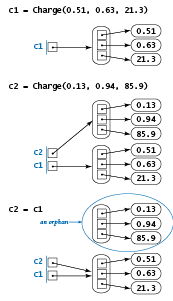
\includegraphics[scale=0.45]{figures/orphaning.png}

\smallskip

\tiny Orphaning an object
\end{center}
\end{minipage}
\end{frame}
\end{document}
